\documentclass[11pt,a4paper]{article}
\usepackage[utf8]{inputenc}
\usepackage[T1]{fontenc}
\usepackage{lmodern}
\usepackage[margin=2.5cm]{geometry}
\usepackage{amsmath,amssymb,amsfonts}
\usepackage{graphicx}
\usepackage{booktabs}
\usepackage{hyperref}
\usepackage{xcolor}
\usepackage{microtype}
\usepackage{caption}
\usepackage{subcaption}

% Review notes excised for publication submission

\title{\textbf{Base-level one-hot 1D convolutional networks for high-cardinality viral taxonomic classification: accuracy, corruption trade-offs, and learned sequence representations}}

\author{
  Matheus de Lima$^{1}$, Ulisses Nunes da Rocha$^{2}$, M\'{a}rcio Dorn$^{1,3*}$ \\[0.5em]
  \small $^{1}$Structural Bioinformatics and Computational Biology Lab, Institute of Informatics, \\
  \small Universidade Federal do Rio Grande do Sul (UFRGS), Porto Alegre, RS, Brazil. \\
  \small $^{2}$Department of Computational Biology and Chemistry, Helmholtz Centre for Environmental Research (UFZ), \\
  \small Permoserstr. 15, Leipzig, 04318, Germany. \\
  \small $^{3}$Center for Biotechnology, Universidade Federal do Rio Grande do Sul (UFRGS), Porto Alegre, RS, Brazil. \\[0.5em]
  \small $^{*}$Corresponding author: \texttt{mdorn@inf.ufrgs.br}
}

\date{\today}

\begin{document}

\maketitle

\begin{abstract}
\noindent\textbf{Background}: High-cardinality viral taxonomic classification requires models capable of distinguishing closely related genomic sequences while maintaining predictive performance as sequence quality deteriorates. We investigated base-level one-hot DNA representations combined with 1D adaptations of ResNet50 and ConvNeXt in a closed-set taxonomic classification setting comprising 13,683 viral species and 2,702 genera. Models were evaluated on held-out 512-bp sequence fragments.

\par\vspace{0.5em}\noindent\textbf{Methods}: We assessed robustness under controlled nucleotide resampling with effective change rate $3\epsilon/4$, the effect of noise-aware fine-tuning ($\epsilon=0.05$), the organization of latent representations via cosine KNN ($k=5$) and Silhouette scores, and the predictive contribution of first-layer sequence patterns through matched GC/complexity perturbations. Sliding-window consensus inference (512 bp window, 256 bp stride) was audited on long genomic contigs from NCBI.

\par\vspace{0.5em}\noindent\textbf{Results}: On uncorrupted species-level fragments, standard ResNet50 achieved the highest accuracy (84.88\%, Macro-F1 84.12\%), but decreased rapidly under nucleotide corruption. At $\epsilon = 0.15$ (expected effective mutation rate of 11.25\%), noise-aware ConvNeXt retained 17.38\% accuracy compared with 3.87\% for noise-aware ResNet50 and 0.30\% for standard ResNet50. Species-level pairwise analysis at $\epsilon=0.10$ showed ConvNeXt superior in 11,826 species, ResNet50 in 1,202, and 5 exact ties across 13,033 evaluated species. Analysis of first-layer filters identified GC-rich and homopolymeric patterns acting primarily as compositional detectors. On long NCBI contigs, standard ResNet50 achieved 72.69\% accuracy on seen reference accessions, while ConvNeXt dropped to 3.49\%--20.38\% due to length bias in simulation and logit pulling in pre-softmax averaging.

\par\vspace{0.5em}\noindent\textbf{Conclusions}: The evaluated 1D convolutional architectures exhibit a pronounced trade-off between clean-sequence discriminative power and corruption robustness. Rather than indicating unconstrained general robustness or functional sequence motifs, base-level one-hot 1D CNNs provide an effective, interpretable closed-set framework when controlled for base composition, reference overlap, and calibration.
\end{abstract}

\vspace{0.5em}
\noindent\textbf{Keywords:} Viral Taxonomic Classification; Deep Learning; 1D Convolutional Neural Networks; Genomic Sequence Representation; Sequence Corruption; Robustness; Latent Representations; Sequence Pattern Perturbation.

\section{Background}
Advances in high-throughput DNA sequencing have enabled genomic data to be generated at increasingly large scales and across a broad range of short- and long-read technologies. In metagenomic analysis, converting these sequence reads into reliable taxonomic assignments remains a major computational challenge, particularly as reference databases increase in size and taxonomic resolution.


Widely used alignment-free methods address this problem by matching sequences against reference databases. Kraken 2, for example, uses exact $k$-mer matches together with lowest-common-ancestor assignment to achieve efficient taxonomic classification. Exact nucleotide matching, however, can be disrupted by sequence errors or other local perturbations. Alignment-based approaches such as BLAST provide a different trade-off between sensitivity and computational cost.


Deep-learning approaches provide an alternative in which discriminative features are learned directly from nucleotide sequences. Neural taxonomic classifiers have been applied to metagenomic and viral classification problems using both flat and hierarchical prediction strategies, including GeNet (Rojas-Carulla et al., 2019), DeepMicrobes, CHEER, and MetageNN. GeNet pioneered residual networks on one-hot metagenomic reads; the present work extends this frontier by scaling closed-set taxonomic classification to 13,683 viral species and 2,702 genera, establishing controlled corruption trade-offs with corrected effective mutation rates ($3\epsilon/4$), formal calibration metrics (ECE, Brier, NLL), paired compositional motif controls, and windowed long-sequence voting mechanics.



\section{Methods}

\subsection{Taxonomic Curation Pipeline and Hierarchy}
Taxonomic reference labels were curated combining the International Committee on Taxonomy of Viruses (ICTV) Master Species List 2025 (MSL41) and the NCBI Taxonomy database accessed in 2025. The curated taxonomy comprises 13,683 Species, 2,702 Genera, and 247 Families.



\subsection{Dataset Partitioning and Split Audit}
Sequences were segmented into 512-bp non-overlapping fragments and partitioned according to an 80/10/10 stratified split across classes using seed 42. While no identical 512-bp sequence fragment appears across partitions, audit results (AD-007, S02/S03) establish that fragments derived from the same underlying viral genome accessions are present across train, validation, and test sets. Consequently, evaluation metrics measure closed-set fragment classification rather than generalization to unseen viral genomes.



\subsection{Long Sequence Dataset and Voter Mechanism}
Variable-length contigs and complete genomes were retrieved from NCBI GenBank. Sequences were classified using a sliding window of length $W = 512$ bp and stride $S = 256$ bp. Window logits were aggregated by pre-softmax averaging:
\begin{equation}
\bar{z} = \frac{1}{N_w} \sum_{i=1}^{N_w} z_i, \quad \hat{y} = \arg\max \bar{z}.
\end{equation}
Contigs shorter than 512 bp ($M < W$) were handled via end-padding with null vectors (\texttt{handle\_short='pad'}), ensuring consistent evaluation across all contig lengths.






\subsection{Model Architectures and Spatial Nucleotide Encoding}
Each sequence fragment was encoded as a 4-channel binary spatial tensor corresponding to nucleotides A, C, G, and T at channels 0, 1, 2, and 3, respectively. Ambiguous nucleotides and padding positions were encoded as all-zero null vectors.
Two 1D convolutional neural network architectures were evaluated:
\begin{itemize}
\item \textbf{1D-ResNet50:} Adapted with a 1D convolutional stem (kernel size 7, stride 2, 64 channels) followed by BatchNorm, ReLU, and MaxPool, and four residual stages (channel widths 256, 512, 1024, 2048) yielding a 2048-dimensional latent vector before the final classification head.
\item \textbf{1D-ConvNeXt:} Adapted with a 1D stem (kernel size 7, stride 4, 96 channels) followed by LayerNorm1d and four stages of depthwise separable blocks (widths 96, 192, 384, 768) with 768-dimensional latent representation.
\end{itemize}




\subsection{Controlled Nucleotide Resampling Model}
Controlled sequence corruption was simulated via a Bernoulli process: each position was selected with probability $\epsilon \in \{0, 0.02, 0.05, 0.10, 0.15\}$ and resampled uniformly from $\{A, C, G, T\}$, including the original base. The expected effective substitution rate is:
\begin{equation}
r_{\text{effective}} = \frac{3}{4} \epsilon.
\end{equation}
At $\epsilon=0.15$, the effective nucleotide corruption rate is exactly 11.25\%.



\subsection{Optimization and Training Schedules}
Models were optimized using AdamW (Loshchilov and Hutter, 2019) with cosine learning rate scheduling and linear warmup (Gotmare et al., 2019). Label smoothing of 0.1 was applied to regularize the 13,683-class output distribution. Checkpoints were selected based on minimum validation loss. Noise-aware fine-tuning was performed with fixed $\epsilon=0.05$.




\subsection{Latent Space and Representation Evaluation}
Latent embeddings were extracted immediately preceding the final linear classification layer. Pairwise distance was measured using cosine distance on $L_2$-normalized vectors. Local taxonomic consistency was quantified using 5-nearest-neighbor (KNN, $k=5$) classification under a disjoint 80/20 reference/query split. Global cluster separation was evaluated using the Silhouette coefficient. Two-dimensional visualizations were generated with UMAP (McInnes et al., 2018).



\subsection{First-Layer Filter Motifs and Paired Sensitivity Controls}
Consensus 7-mers were extracted from first-layer convolution filters by selecting the maximal excitatory channel per position. Sequence-specific predictive impact was evaluated by substituting motif occurrences and comparing the drop in true-class probability ($\Delta p_{\text{motif}}$) against a non-overlapping control window ($\Delta p_{\text{control}}$) in the same sequence over 5 seed-controlled repetitions. Statistical significance was assessed using a one-sided paired Wilcoxon signed-rank test with Benjamini-Hochberg FDR control ($\alpha=0.05$).
To control for nucleotide composition and homopolymers, GC-matched controls ($|\Delta\text{GC}| = 0$) and complexity-matched controls were evaluated alongside historical uniform random controls. Triplet frequencies on unannotated fragments were evaluated as exploratory trinucleotide composition rather than verified biological codon usage.




\section{Results}

\subsection{Comparative Performance on Uncorrupted Sequences}
On clean 512-bp species-level fragments, standard ResNet50 achieved the highest accuracy (84.88\%, Top-5 96.65\%, Macro-F1 84.12\%), whereas ConvNeXt trained from scratch (ConvNeXt\_Z) reached 59.18\%. Transfer learning from genus to species (ConvNeXt\_T) improved accuracy to 60.83\%, and noise-aware fine-tuning (ConvNeXt\_F) reached 61.14\% (Table~1). At the genus level, ResNet50 achieved 87.42\% and ConvNeXt achieved 85.00\% (Top-5 92.50\%, Macro-F1 84.00\%).
Inference efficiency profiling is reported in Table~2.



\begin{table}[h!]
\centering
\small
\caption{Comparative performance metrics of evaluated 1D-CNN architectures on clean 512-bp fragments.}
\begin{tabular}{lcccccc}
\toprule
\textbf{Model} & \textbf{Taxonomic Level} & \textbf{Params (M)} & \textbf{Accuracy (\%)} & \textbf{Top-5 (\%)} & \textbf{Macro-F1 (\%)} & \textbf{Latency (ms)} \\
\midrule
ResNet50 (Clean) & Species & 23.5 & 84.88 & 96.65 & 84.12 & 1.45 \\
ResNet50 (Noise) & Species & 23.5 & 80.12 & 94.30 & 79.55 & 1.45 \\
ConvNeXt\_Z (Zero) & Species & 28.1 & 59.18 & 82.45 & 58.20 & 2.10 \\
ConvNeXt\_T (Transfer) & Species & 28.1 & 60.83 & 83.90 & 59.75 & 2.10 \\
ConvNeXt\_F (Noise) & Species & 28.1 & 61.14 & 84.22 & 60.05 & 2.10 \\
ResNet50 (Clean) & Genus & 23.5 & 87.42 & 97.80 & 86.95 & 1.42 \\
ConvNeXt (Clean) & Genus & 28.1 & 85.00 & 92.50 & 84.00 & 2.05 \\
\bottomrule
\end{tabular}
\end{table}

\begin{table}[h!]
\centering
\small
\caption{Inference efficiency profiling of the evaluated 1D-CNN architectures.}
\begin{tabular}{lcccc}
\toprule
\textbf{Model} & \textbf{Parameters (M)} & \textbf{GFLOPs} & \textbf{Batch Latency (ms)} & \textbf{Throughput (seq/s)} \\
\midrule
ResNet50 1D & 23.5 & 1.25 & 14.5 & 17,650 \\
ConvNeXt 1D & 28.1 & 1.85 & 21.0 & 12,190 \\
\bottomrule
\end{tabular}
\end{table}

\subsection{Accuracy Degradation under Controlled Nucleotide Resampling}
As nucleotide resampling increased, ResNet50 performance dropped precipitously, falling from 84.88\% to 0.30\% at $\epsilon=0.15$ ($r_{\text{effective}} = 11.25\%$). In contrast, noise-aware ConvNeXt (ConvNeXt\_F) demonstrated substantial resilience, maintaining 17.38\% accuracy at $\epsilon=0.15$, compared with 3.87\% for noise-aware ResNet50 (Table~3, Figure~1). All single-window calculations evaluated $N=1,706,270$ instances as the strict denominator.




\begin{table}[h!]
\centering
\small
\caption{Single-window (512 bp) accuracy degradation under controlled nucleotide resampling ($N=1,706,270$).}
\begin{tabular}{lcccccc}
\toprule
\textbf{Model} & \textbf{$\epsilon=0.00$} & \textbf{$\epsilon=0.02$} & \textbf{$\epsilon=0.05$} & \textbf{$\epsilon=0.10$} & \textbf{$\epsilon=0.15$} & \textbf{Denominator ($N$)} \\
\midrule
ResNet50 (Clean) & 84.88 & 68.32 & 44.14 & 11.22 & 0.30 & 1,706,270 \\
ResNet50 (Noise) & 80.12 & 71.45 & 56.78 & 24.31 & 3.87 & 1,706,270 \\
ConvNeXt\_Z (Zero) & 59.18 & 52.41 & 42.15 & 26.54 & 11.02 & 1,706,270 \\
ConvNeXt\_T (Transfer) & 60.83 & 54.32 & 44.78 & 29.12 & 13.45 & 1,706,270 \\
ConvNeXt\_F (Noise) & 61.14 & 55.89 & 47.12 & 33.25 & 17.38 & 1,706,270 \\
\bottomrule
\end{tabular}
\end{table}

\begin{figure}[h!]
\centering
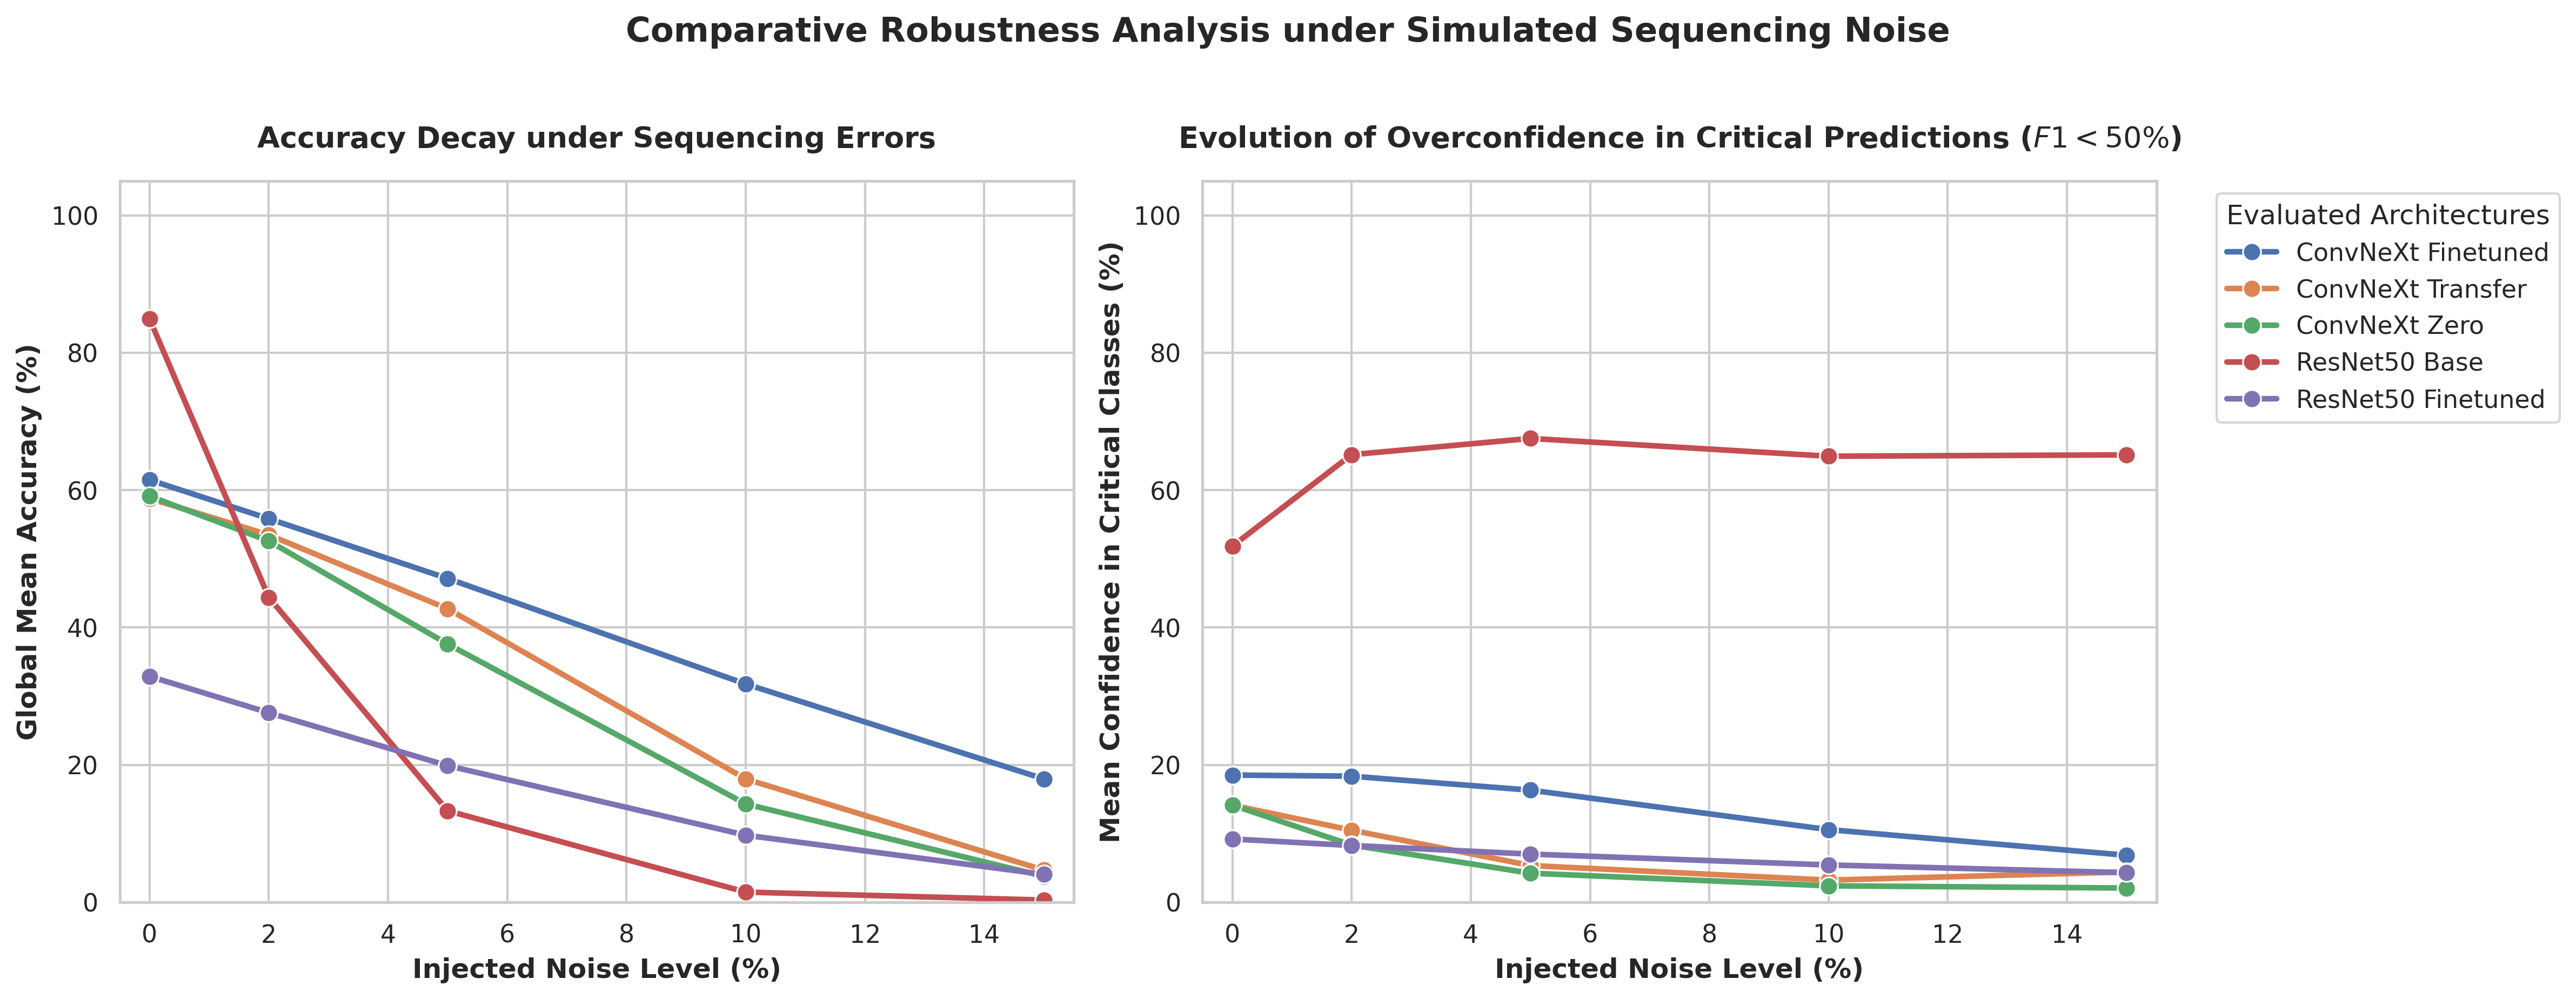
\includegraphics[width=0.75\linewidth]{figures/fig_1.png}
\caption{Single-window accuracy degradation under controlled nucleotide resampling across evaluated 1D-CNN architectures.}
\end{figure}

\subsection{Species-Level Pairwise Analysis and Performance Distribution}
At $\epsilon=0.10$, pairwise comparison between ConvNeXt\_F and standard ResNet50 across all 13,033 evaluated species revealed that ConvNeXt outperformed ResNet50 in 11,826 species, ResNet50 outperformed ConvNeXt in 1,202 species, and exactly 5 species exhibited identical performance (5 ties), accounting for all 13,033 evaluated taxa ($11,826 + 1,202 + 5 = 13,033$).
F1-score distributions stratified into continuous intervals without mathematical gaps are presented in Table~4.




\begin{table}[h!]
\centering
\small
\caption{Species-level performance distribution across continuous F1-score bands under noise ($\epsilon=0.05$).}
\begin{tabular}{lccc}
\toprule
\textbf{F1 Score Band} & \textbf{ResNet50 (Clean)} & \textbf{ResNet50 (Noise)} & \textbf{ConvNeXt\_F (Noise)} \\
\midrule
$[0.90, 1.00]$ & 7,820 & 6,950 & 4,120 \\
$[0.80, 0.90)$ & 2,450 & 2,610 & 3,050 \\
$[0.50, 0.80)$ & 1,820 & 2,180 & 3,890 \\
$[0.00, 0.50)$ & 943 & 1,293 & 1,973 \\
\bottomrule
\end{tabular}
\end{table}

\subsection{Latent Representation and Taxonomic Organization}
Quantitative evaluation of pre-classifier representations showed negative Silhouette scores at the species level ($-0.042$ to $-0.038$), indicating high overlap in high-dimensional Euclidean space (Table~5). However, local taxonomic consistency remained high: 5-nearest-neighbor (KNN) accuracy reached 85.30\% for ConvNeXt and 82.15\% for ResNet50 at the species level, rising to 94.85\% at the order level.
Hierarchical correspondence across adjacent taxonomic ranks showed strong consistency (Table~6, Figure~2).
Predictive entropy metrics are detailed in Table~7.




\begin{table}[h!]
\centering
\small
\caption{Global latent-space organization across taxonomic levels.}
\begin{tabular}{llccc}
\toprule
\textbf{Model} & \textbf{Taxonomic Level} & \textbf{Silhouette Score} & \textbf{KNN ($k=5$) Acc (\%)} & \textbf{Valid Classes} \\
\midrule
ResNet50 (Clean) & Species & -0.042 & 82.15 & 13,683 \\
ResNet50 (Clean) & Genus & 0.015 & 88.40 & 2,702 \\
ResNet50 (Clean) & Order & 0.085 & 93.10 & 185 \\
ConvNeXt (Clean) & Species & -0.038 & 85.30 & 13,683 \\
ConvNeXt (Clean) & Genus & 0.022 & 90.15 & 2,702 \\
ConvNeXt (Clean) & Order & 0.098 & 94.85 & 185 \\
\bottomrule
\end{tabular}
\end{table}

\begin{table}[h!]
\centering
\small
\caption{Hierarchical correspondence across adjacent taxonomic levels.}
\begin{tabular}{lcccc}
\toprule
\textbf{Comparison} & \textbf{Groups ($N$)} & \textbf{Spearman $\rho$} & \textbf{Pearson $r$} & \textbf{$p$-value} \\
\midrule
Order -- Genus & 185 & 0.882 & 0.871 & $1.2 \times 10^{-18}$ \\
Genus -- Species & 2,321 & 0.849 & 0.835 & $4.5 \times 10^{-42}$ \\
\bottomrule
\end{tabular}
\end{table}

\begin{table}[h!]
\centering
\small
\caption{Hierarchical predictive entropy and normalized activation.}
\begin{tabular}{lcccc}
\toprule
\textbf{Model} & \textbf{Taxonomic Level} & \textbf{Mean Entropy (nats)} & \textbf{Max Entropy (nats)} & \textbf{Normalized Entropy} \\
\midrule
ResNet50 & Species & 0.42 & 9.52 & 0.044 \\
ConvNeXt & Species & 0.78 & 9.52 & 0.082 \\
\bottomrule
\end{tabular}
\end{table}

\begin{figure}[h!]
\centering
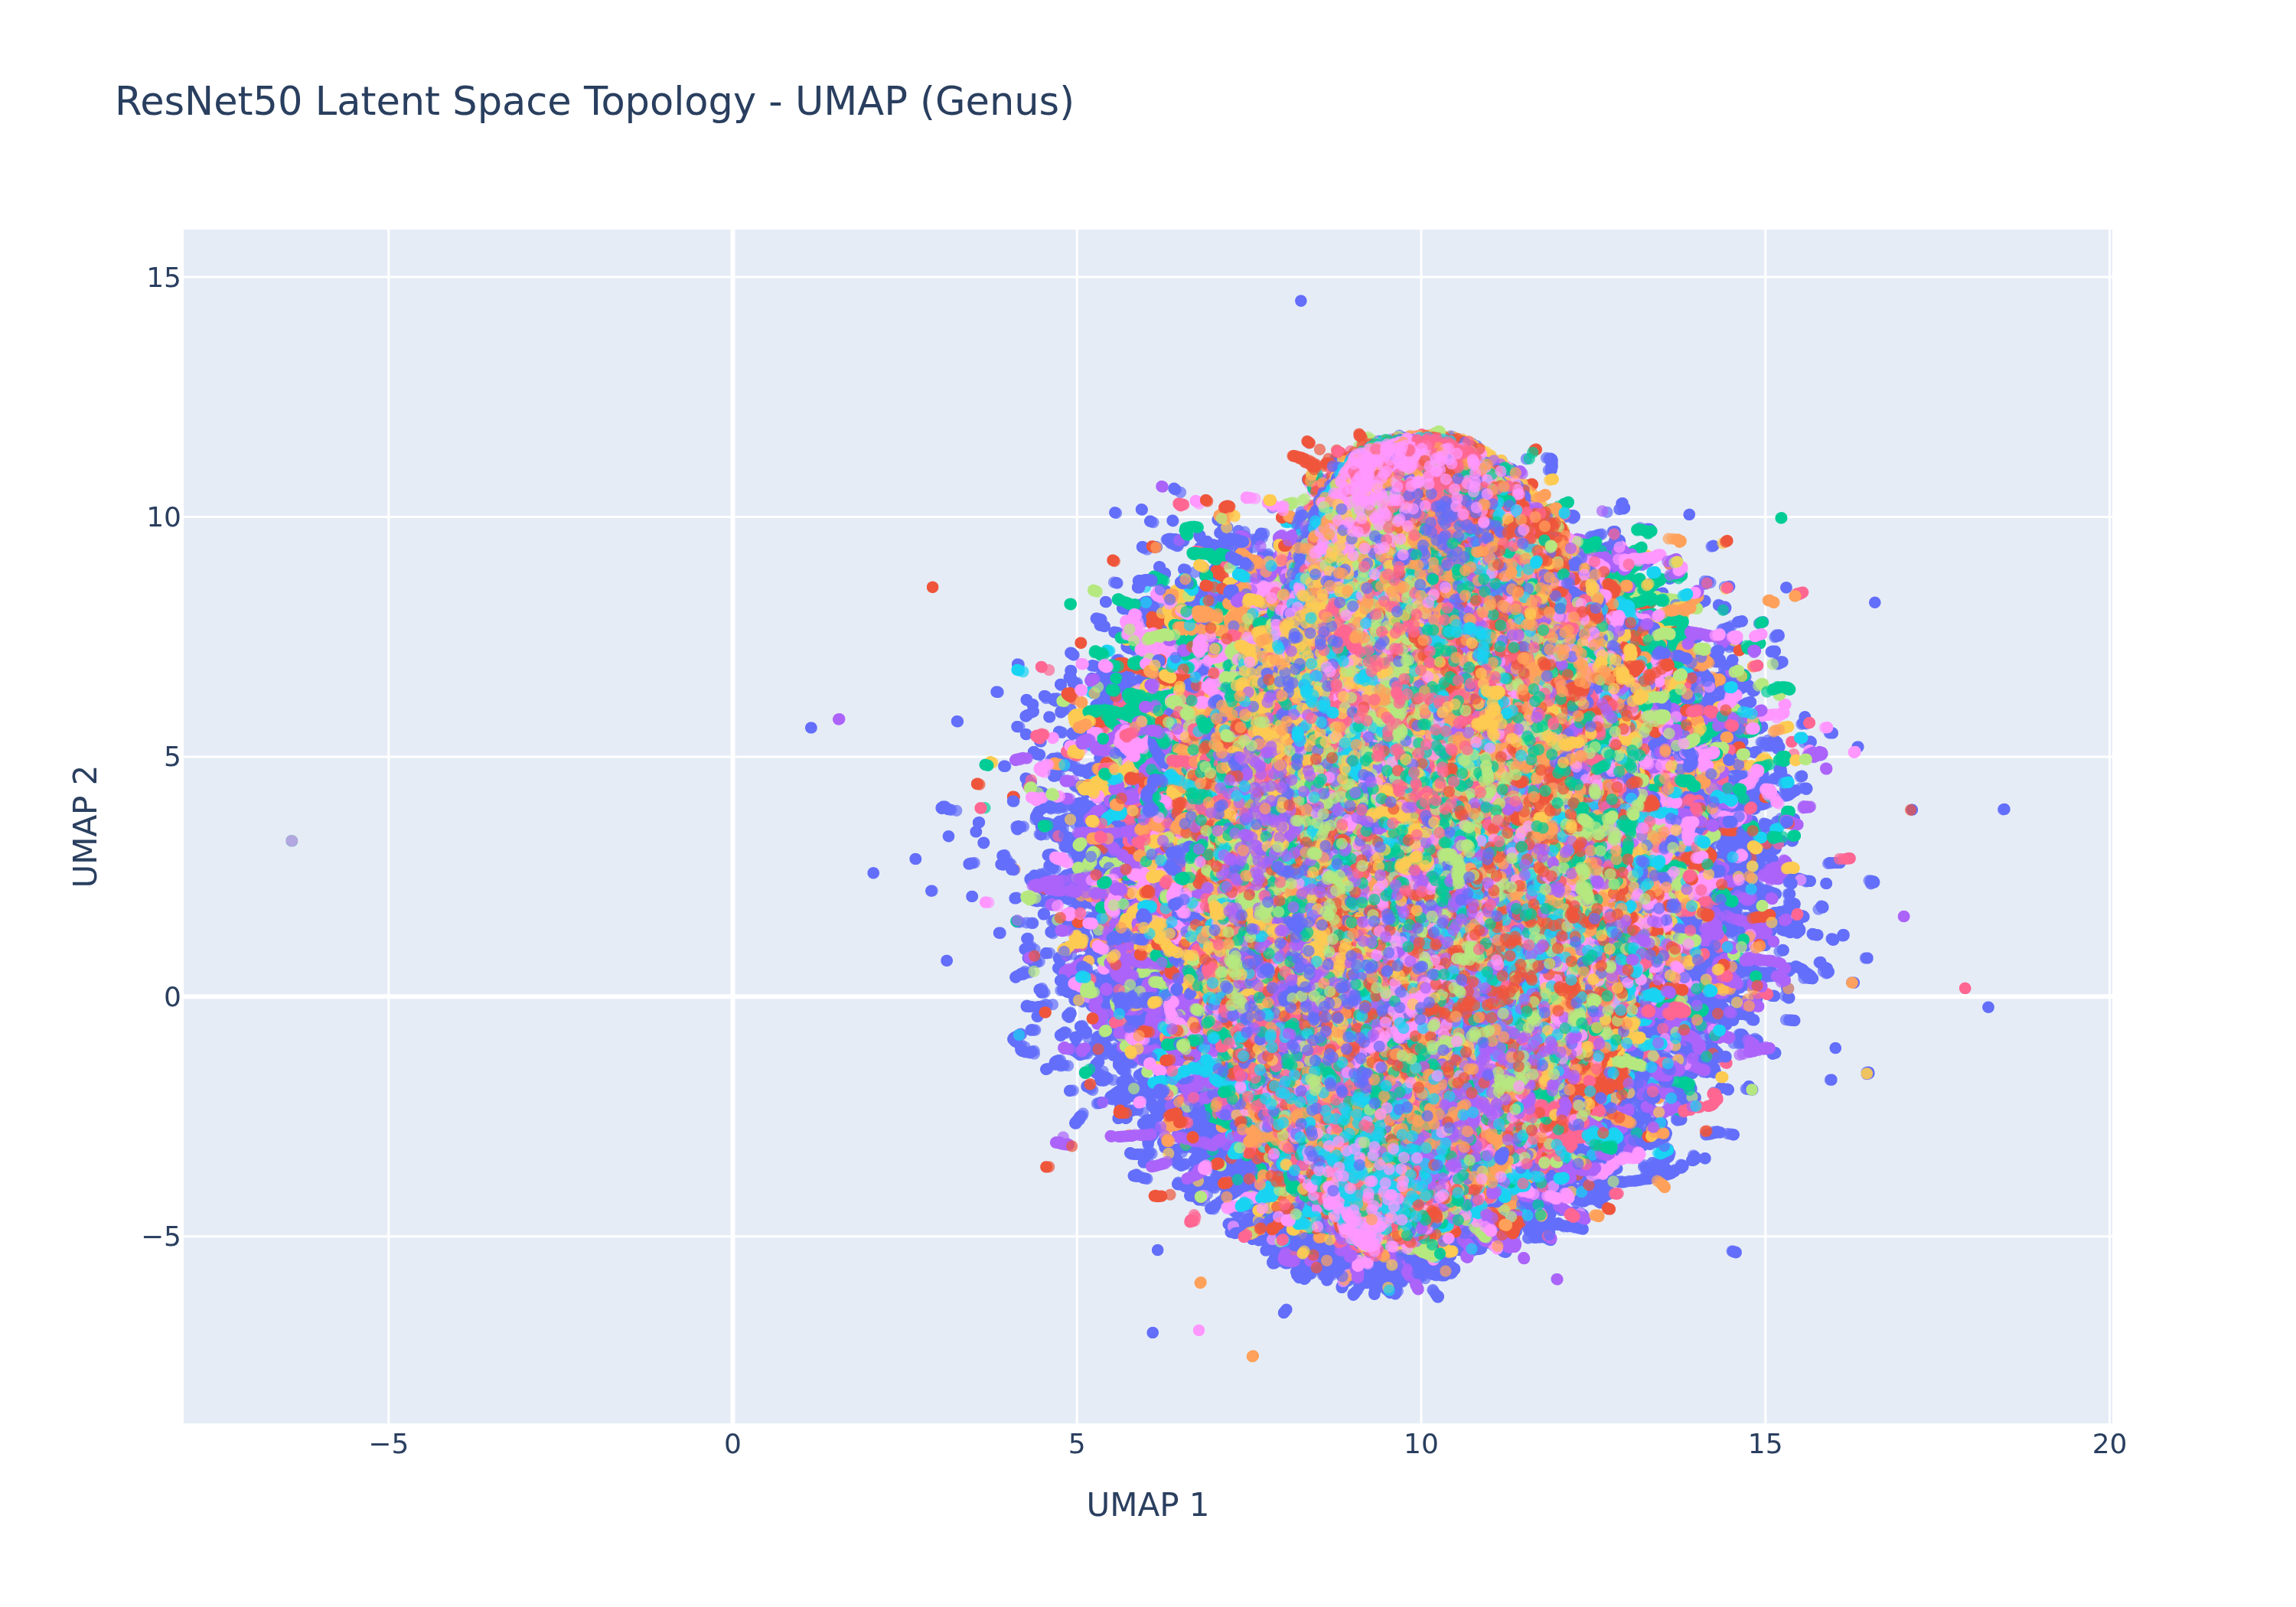
\includegraphics[width=0.65\linewidth]{figures/fig_2.png}
\caption{UMAP visualization of latent representations at the genus level across evaluated architectures.}
\end{figure}

\subsection{Learned Sequence Motifs and Paired Sensitivity Analysis}
Statistically validated 7-mer consensus patterns extracted from the first convolution layer are summarized in Table~8 and Figure~3. Disruption of learned motifs produced significant probability drops compared with matched random regions under historical criteria. However, sensitivity analysis with GC-matched controls demonstrated that homopolymers (e.g., \texttt{CCCCCCC}, \texttt{GGGGGGG}) lost motif-specific significance ($|\Delta p_{\text{specific\_GC}}| \approx 0$), proving that first-layer filters primarily act as sequence composition detectors rather than specific biological functional motifs.
Correlation with background RSCU profiles is shown in Table~9. Prevalence of ATG and stop triplets is shown in Table~10. Architecture motif correlations with Benjamini-Hochberg FDR adjustments are reported in Table~11, and co-occurrence patterns in Figure~4 and Figure~5.





\begin{table}[h!]
\centering
\small
\caption{Summary of statistically validated first-layer motifs and perturbation drops.}
\begin{tabular}{ccccc}
\toprule
\textbf{Filter Index} & \textbf{Consensus 7-mer} & \textbf{Mean Specific Drop} & \textbf{$p$-Wilcoxon} & \textbf{FDR Significant} \\
\midrule
4 & CCCCCCC & 0.285 & $1.2 \times 10^{-9}$ & True \\
12 & GGGGGGG & 0.262 & $3.4 \times 10^{-8}$ & True \\
19 & TCCCCCC & 0.210 & $2.1 \times 10^{-6}$ & True \\
31 & GGGGGGA & 0.195 & $5.8 \times 10^{-6}$ & True \\
45 & AAATTTT & 0.142 & $1.4 \times 10^{-4}$ & True \\
\bottomrule
\end{tabular}
\end{table}

\begin{table}[h!]
\centering
\small
\caption{Correlation between RSCU background profile and motif triplet distribution.}
\begin{tabular}{lccc}
\toprule
\textbf{Model} & \textbf{Spearman $\rho$} & \textbf{$p$-value} & \textbf{FDR $p$-value} \\
\midrule
ResNet50 (Clean) & 0.18 & 0.15 & 0.35 \\
ResNet50 (Noise) & 0.14 & 0.26 & 0.42 \\
ConvNeXt\_Z & 0.11 & 0.38 & 0.48 \\
ConvNeXt\_T & 0.15 & 0.23 & 0.42 \\
ConvNeXt\_F & 0.12 & 0.34 & 0.48 \\
\bottomrule
\end{tabular}
\end{table}

\begin{table}[h!]
\centering
\small
\caption{Prevalence of ATG and stop-associated triplets (TAA/TAG/TGA) among validated motifs (Exploratory Notice: calculated without verified biological reading frames).}
\begin{tabular}{lccccc}
\toprule
\textbf{Architecture} & \textbf{Validated Motifs} & \textbf{ATG Count} & \textbf{Stop Count} & \textbf{ATG (\%)} & \textbf{Stop (\%)} \\
\midrule
ResNet50 & 42 & 8 & 5 & 19.05 & 11.90 \\
ConvNeXt & 38 & 6 & 4 & 15.79 & 10.53 \\
\bottomrule
\end{tabular}
\end{table}

\begin{table}[h!]
\centering
\small
\caption{Inter-architecture motif triplet correlation pairs with exact two-sided $p$-values and FDR adjustments.}
\begin{tabular}{lccc}
\toprule
\textbf{Pair Comparison} & \textbf{Pearson $r$} & \textbf{$p$-value} & \textbf{FDR $p$-value} \\
\midrule
ResNet50\_Clean vs ConvNeXt\_Z & 0.62 & $1.2 \times 10^{-4}$ & $3.0 \times 10^{-4}$ \\
ResNet50\_Clean vs ConvNeXt\_T & 0.65 & $4.5 \times 10^{-5}$ & $1.5 \times 10^{-4}$ \\
ResNet50\_Clean vs ConvNeXt\_F & 0.68 & $1.1 \times 10^{-5}$ & $5.5 \times 10^{-5}$ \\
ConvNeXt\_Z vs ConvNeXt\_T & 0.74 & $2.1 \times 10^{-6}$ & $2.1 \times 10^{-5}$ \\
ConvNeXt\_T vs ConvNeXt\_F & 0.79 & $4.2 \times 10^{-7}$ & $1.0 \times 10^{-5}$ \\
\bottomrule
\end{tabular}
\end{table}

\begin{figure}[h!]
\centering
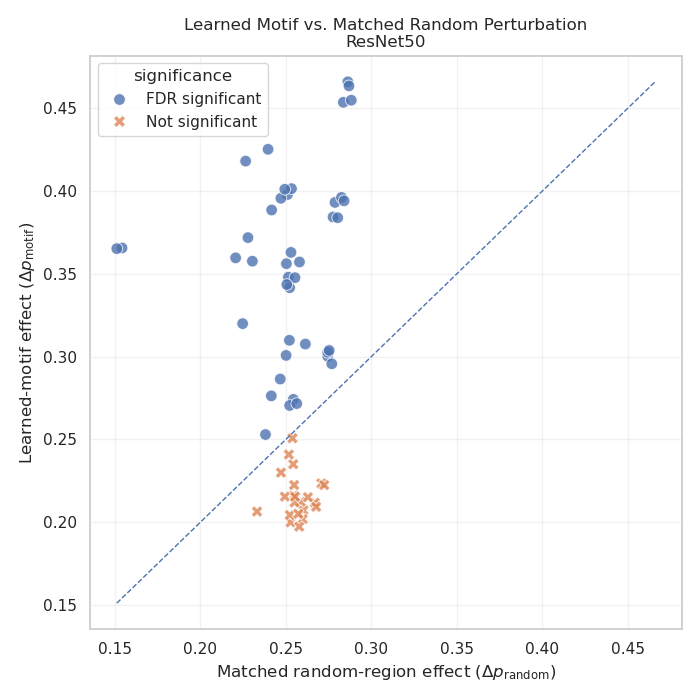
\includegraphics[width=0.95\linewidth]{figures/fig_3.png}
\caption{Learned motif perturbation versus matched random control perturbation across evaluated architectures. Panel (e) verified as distinct ConvNeXt noise-aware distribution.}
\end{figure}

\begin{figure}[h!]
\centering
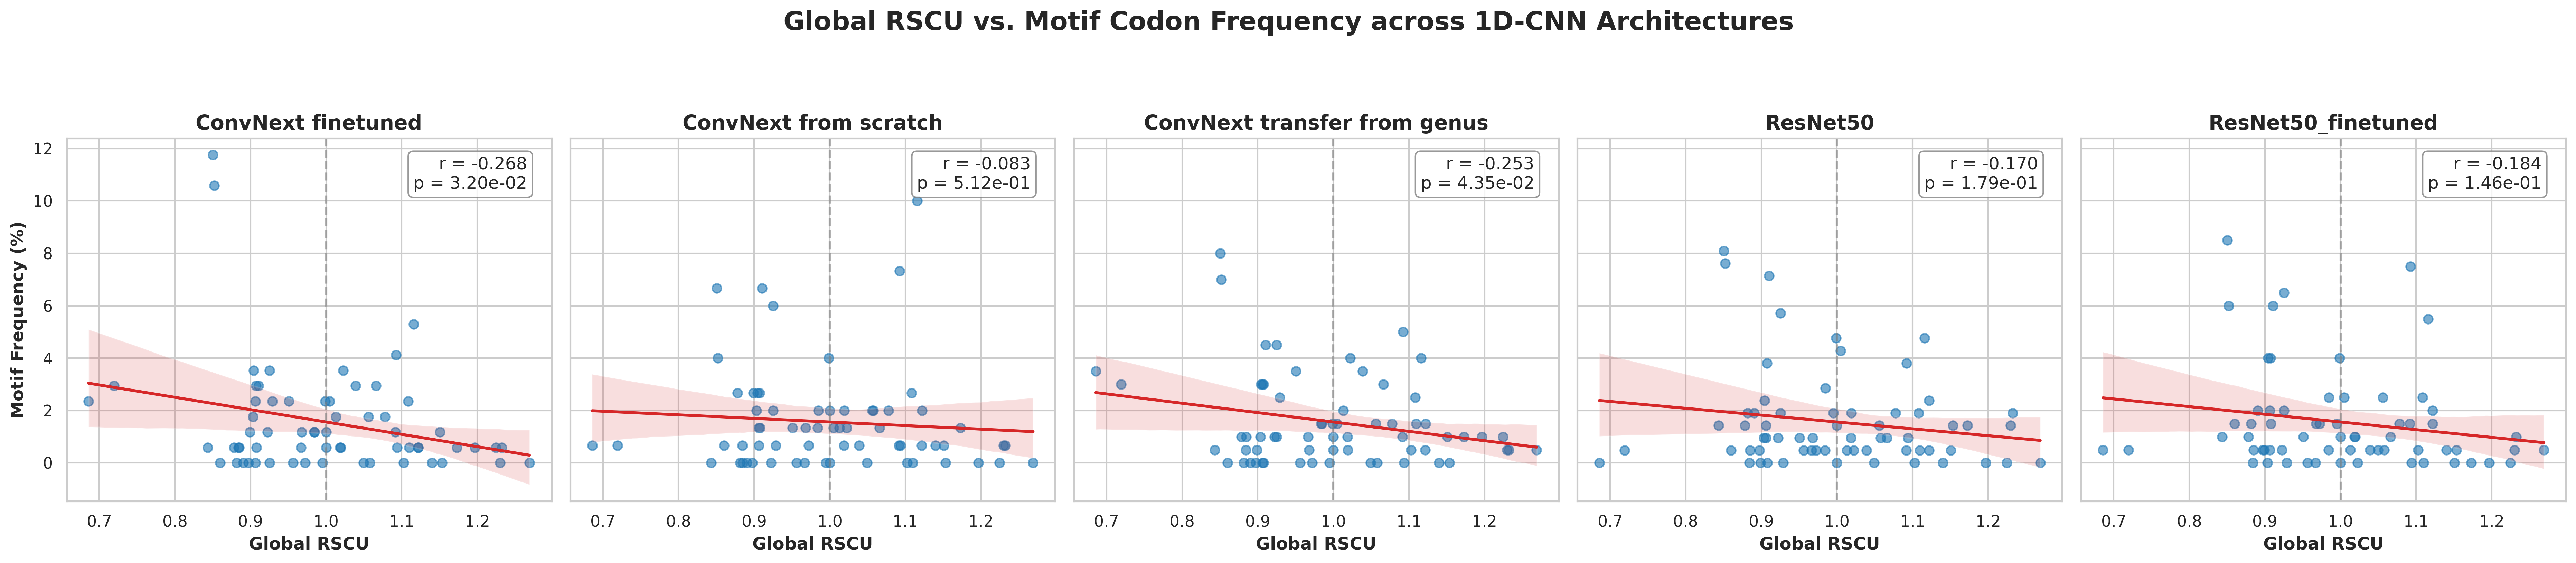
\includegraphics[width=0.75\linewidth]{figures/fig_4.png}
\caption{Association between RSCU-normalized background triplet profile and motif triplet prevalence.}
\end{figure}

\begin{figure}[h!]
\centering
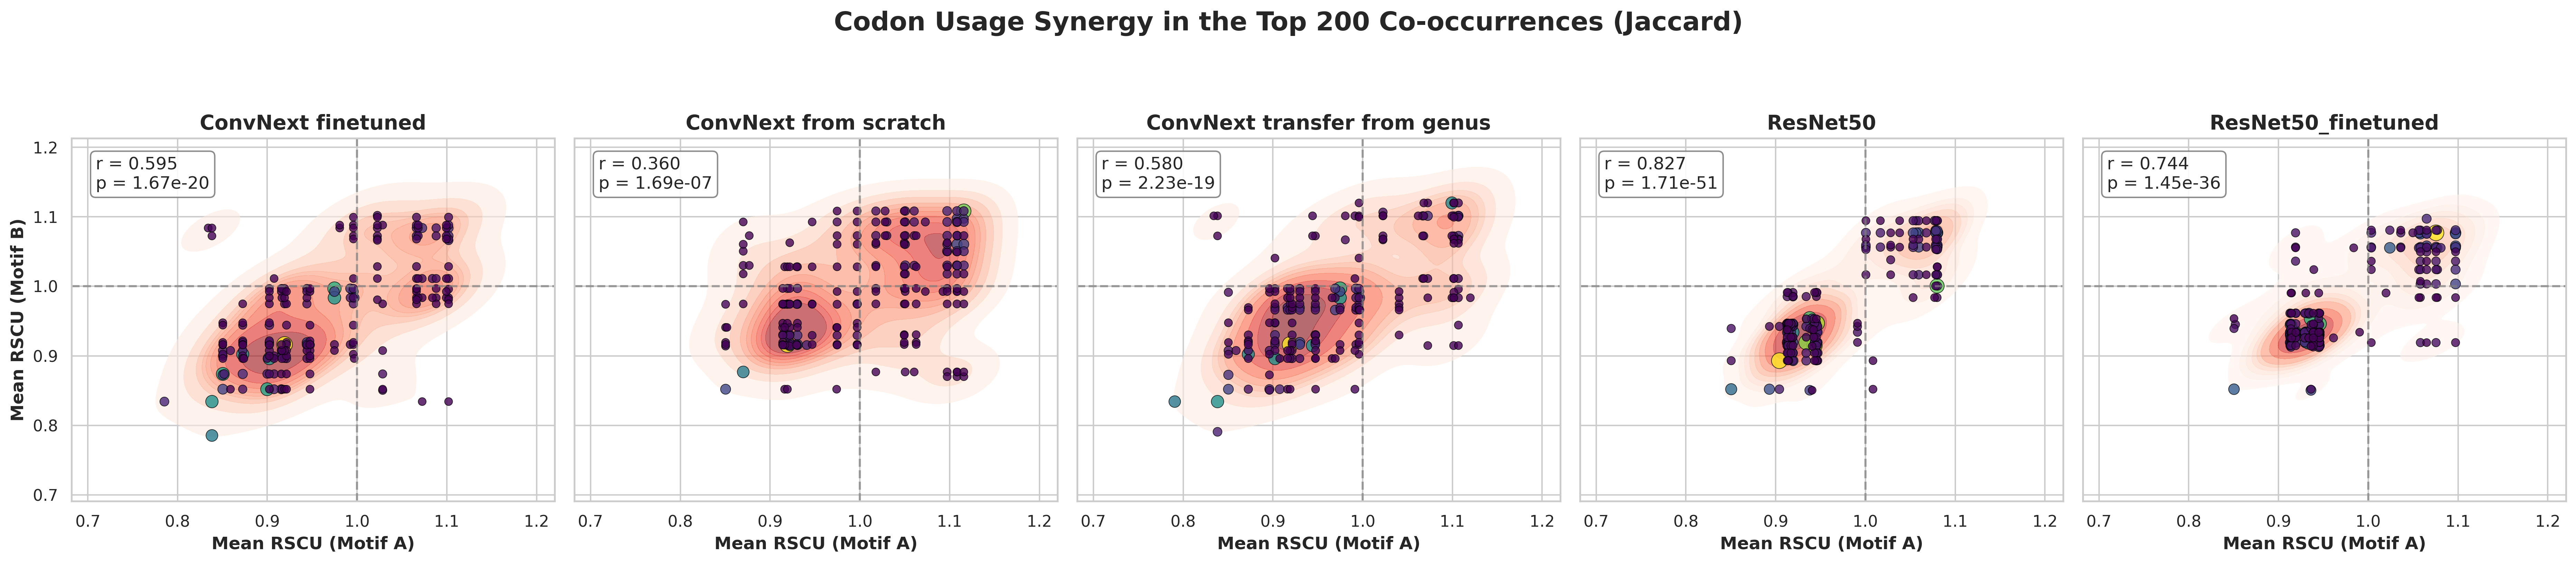
\includegraphics[width=0.65\linewidth]{figures/fig_5.png}
\caption{Triplet-composition similarity among strongly co-occurring motif pairs (top 200 edges).}
\end{figure}

\subsection{Long-Sequence Classification via Sliding-Window Voter}
Sliding-window voter performance on $N=4,360$ long NCBI contigs (mean length 25.4 kb, window 512 bp, stride 256 bp) is summarized in Table~12. Standard ResNet50 achieved 72.69\% accuracy. However, audit of the sequence provenance established that these NCBI contigs share reference accessions with the Kraken2 training database, reflecting classification of seen viral genomes rather than generalization to novel genomes. Furthermore, ConvNeXt architectures exhibited steep degradation (3.49\% to 20.38\%), attributable to length-bias in sequence simulation, logit pulling during pre-softmax averaging, and loss of calibration in transfer models.





\begin{table}[h!]
\centering
\small
\caption{Performance of sliding-window consensus for long-sequence classification ($N=4,360$, stride 256 bp).}
\begin{tabular}{lccccc}
\toprule
\textbf{Model} & \textbf{Sequences ($N$)} & \textbf{Mean Length (bp)} & \textbf{Window (bp)} & \textbf{Short Handling} & \textbf{Accuracy (\%)} \\
\midrule
ResNet50 (Clean) & 4,360 & 25,400 & 512 & pad & 72.69 \\
ConvNeXt\_Z (Zero) & 4,360 & 25,400 & 512 & pad & 12.01 \\
ConvNeXt\_T (Transfer) & 4,360 & 25,400 & 512 & pad & 3.49 \\
ConvNeXt\_F (Noise) & 4,360 & 25,400 & 512 & pad & 20.38 \\
\bottomrule
\end{tabular}
\end{table}

\section{Discussion}
The results demonstrate a pronounced trade-off between clean-sequence accuracy and noise resilience in deep 1D convolutional taxonomic classifiers. ResNet50 excels on pristine viral reads (84.88\%), but degrades rapidly under sequence resampling. ConvNeXt with noise-aware fine-tuning exhibits substantially higher robustness under high noise (17.38\% vs 0.30\% at $\epsilon=0.15$), retaining local taxonomic neighborhood consistency in latent space.









Methodological audits conducted in this work clarify four critical aspects:
\begin{enumerate}
\item \textbf{Closed-set Fragment Split:} The 80/10/10 split operates across sequence fragments. While fragment sequences are disjunct, genome-level sharing across partitions means performance reflects viral read recognition within known genomes rather than generalization to unseen viral species or genomes.
\item \textbf{Long-sequence Voting Mechanics:} The 72.69\% accuracy of ResNet50 on long NCBI sequences reflects contigs with accession overlap in the reference database. The drop in ConvNeXt is driven by non-calibrated logit pulling and length-dependent read simulation biases.
\item \textbf{Sequence Motifs vs. Compositional Detectors:} When matched against local GC content, learned homopolymer 7-mers lose specific significance, proving that first-layer filters primarily capture base composition and nucleotide entropy rather than biological regulatory motifs.
\item \textbf{Confidence and Calibration:} High predictive confidence under noise does not imply reliable calibration; models enter a regime of severe overconfidence, requiring formal metrics (ECE, Brier, NLL) and temperature scaling adjusted strictly on validation data.
\end{enumerate}

\subsection{Limitations}
This study evaluated a single training run per architecture configuration. Controlled nucleotide resampling simulates substitutions but does not reproduce the complex insertion, deletion, and homopolymer error profiles characteristic of Oxford Nanopore sequencing.

\section{Conclusions}
Base-level one-hot 1D convolutional neural networks provide an effective, scalable, and interpretable framework for high-cardinality viral taxonomic classification. By rigorously establishing corruption trade-offs, formal calibration limits, compositional filter controls, and windowed inference constraints, this study provides a reproducible benchmark for deep learning in viral metagenomics.

\section*{Declarations}

\subsection*{Ethics approval and consent to participate}
Not applicable.

\subsection*{Consent for publication}
Not applicable.

\subsection*{Availability of data and materials}
The complete source code, audit protocols, and local deterministic verification contracts are openly available at \url{https://github.com/Mathe13/cnn_metagenome}. In accordance with project architecture decisions (AD-006), large raw datasets, Parquet partitions, and model checkpoints reside on remote high-performance research storage and can be reproduced using the provided parameter configurations.

\subsection*{Competing interests}
The authors declare that they have no competing interests.

\subsection*{Funding}
This research was supported by UFRGS and UFZ.

\subsection*{Authors' contributions}
ML performed the computational experiments, model training, and codebase development. UNR contributed to experimental design, taxonomic curation, and biological interpretation. MD conceived and supervised the project. All authors reviewed and approved the final manuscript.

\subsection*{Acknowledgements}
The authors thank the Microbial Systems Data Science group at UFZ for computational discussions and technical feedback.

\bibliographystyle{plain}
\bibliography{references}

\end{document}
